% ###########################################################################
\section{Experimental Setup and Results}
\label{sec:evaluation_presentation}
% ###########################################################################
This section describes the experimental setup and presents the results comparing
the Linux implementations of TCP and MPTCP for transferring web traffic. We
evaluated the protocols performance through both emulations and real-word experiments, identifying the impact of various network
parameters in both homogeneous and heterogeneous scenarios. 

\begin{figure*}
  \centering
  \begin{tabular}{ccc}
  \subfloat[Wikipedia download, $15$ objects, $72$Kb total size.\label{fig:web:wikipedia}]{
   \includegraphics[width=.28\linewidth]{plots/wikipedia_avgDelay_bar}
  } &
  \subfloat[Amazon download, $54$ objects, $1$Mb total size.\label{fig:web:amazon}]
  {
    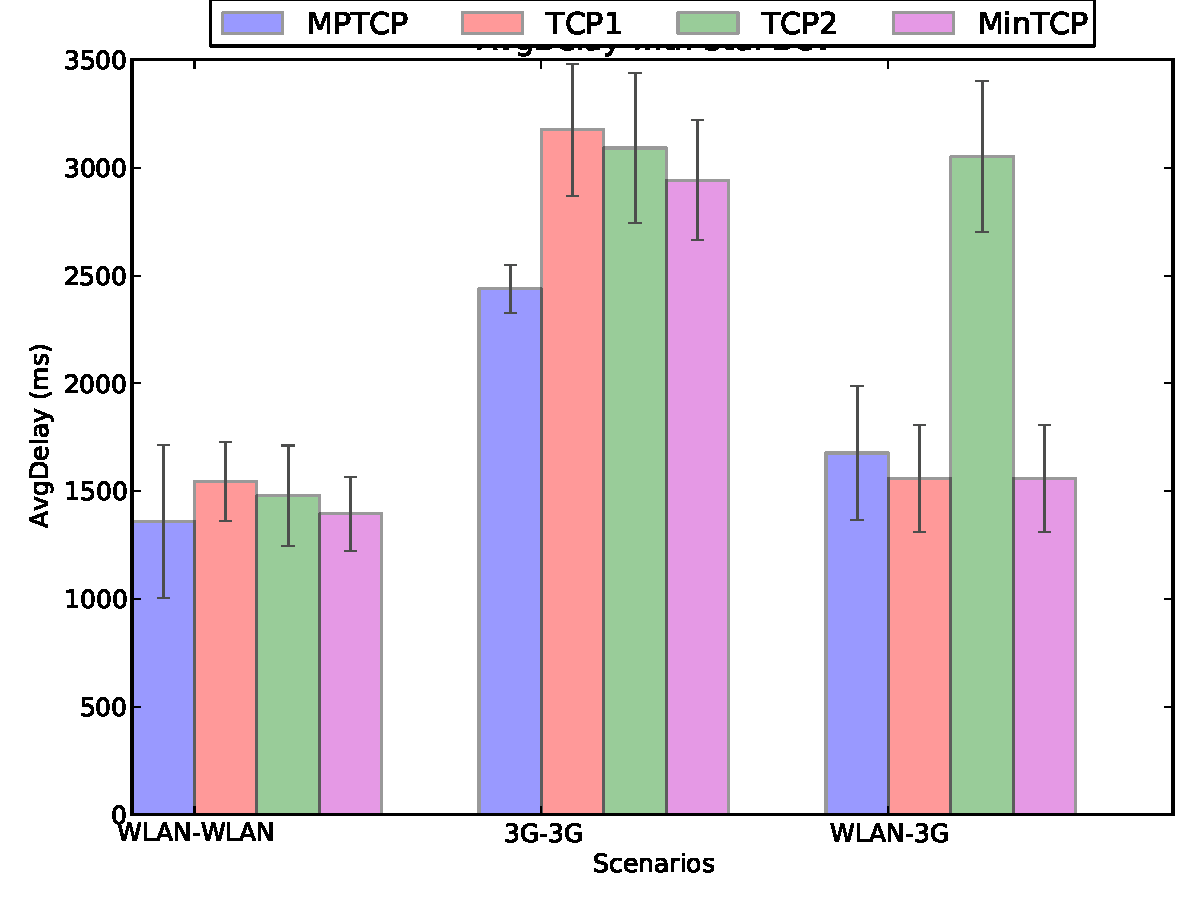
\includegraphics[width=.28\linewidth]{plots/Amazon_avgDelay_bar}
  } &
  \subfloat[Huffington Post download, $134$ objects, $3.9$Mb total size.\label{fig:web:huffpost}]
  {
    \includegraphics[width=.28\linewidth]{plots/huffpost_avgDelay_bar}
  } 
%  \\
%  \subfloat[Wikipedia download, XYZ objects of average size XYZKB.\label{fig:web:wikipediawbg}]{
%	  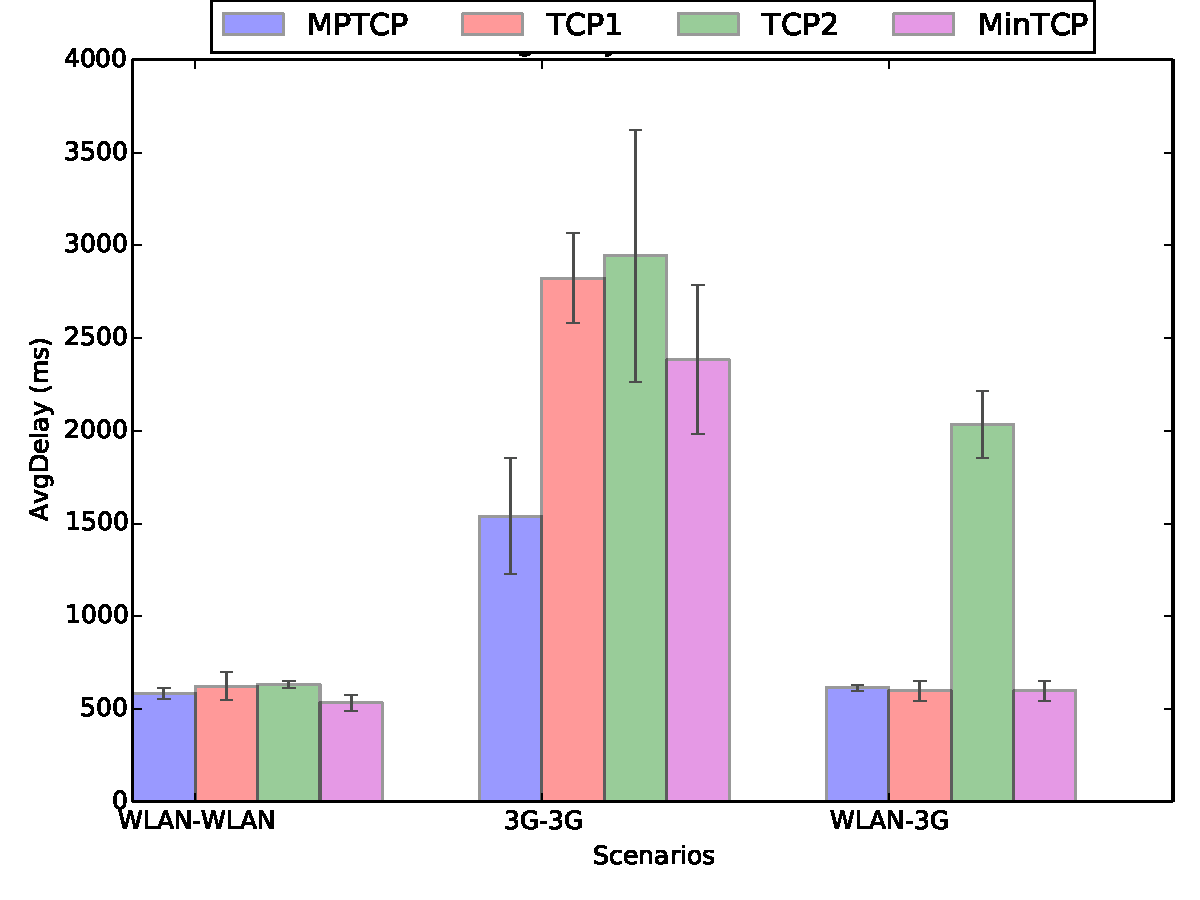
\includegraphics[width=.32\linewidth]{plots/wikipedia_avgDelayWBG}
%  } &
%  \subfloat[Amazon download, XYZ objects of average size XYZKB.\label{fig:web:amazonwbg}]
%  {
%    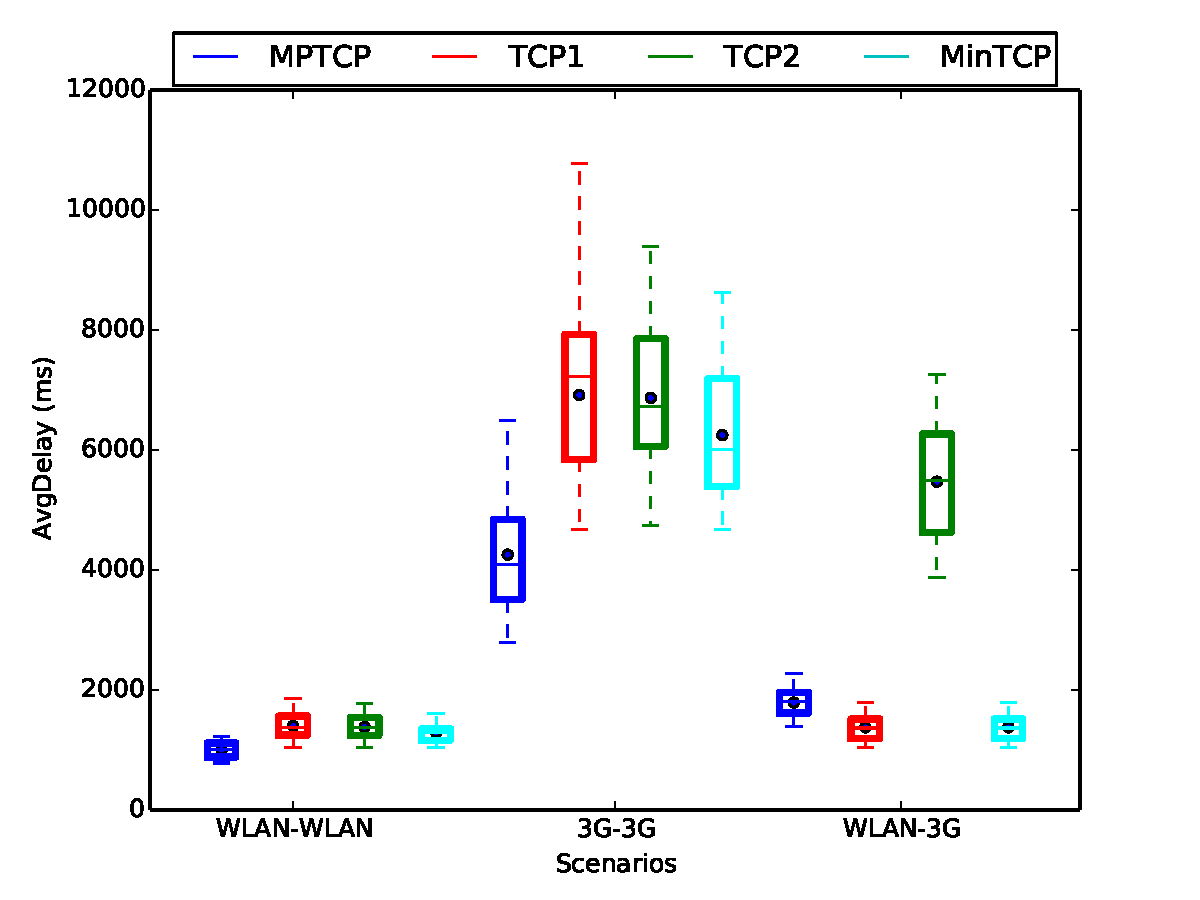
\includegraphics[width=.32\linewidth]{plots/Amazon_avgDelayWBG}
%  } &
%  \subfloat[Huffington Post download, XYZ objects of average size XYZKB.\label{fig:web:huffpostwbg}]
%  {
%    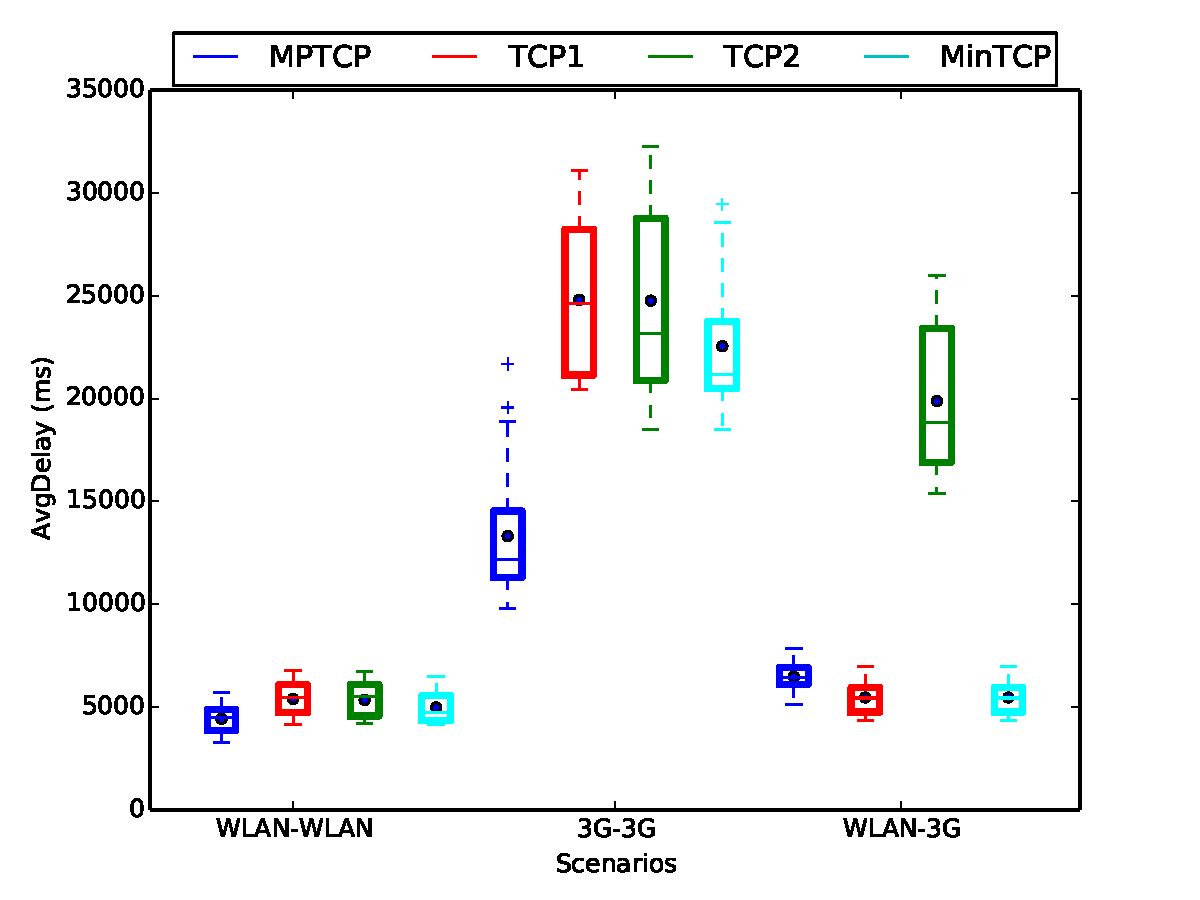
\includegraphics[width=.32\linewidth]{plots/huffpost_avgDelayWBG}
%  }
  \end{tabular}
  \caption{Average web transfer delay, with standard deviation.}
  \label{fig:web}
\end{figure*}

\begin{figure*}
  \centering
  \subfloat[Application Delay: TCP\label{fig:nornet_tcp_http_appdelay}]{
    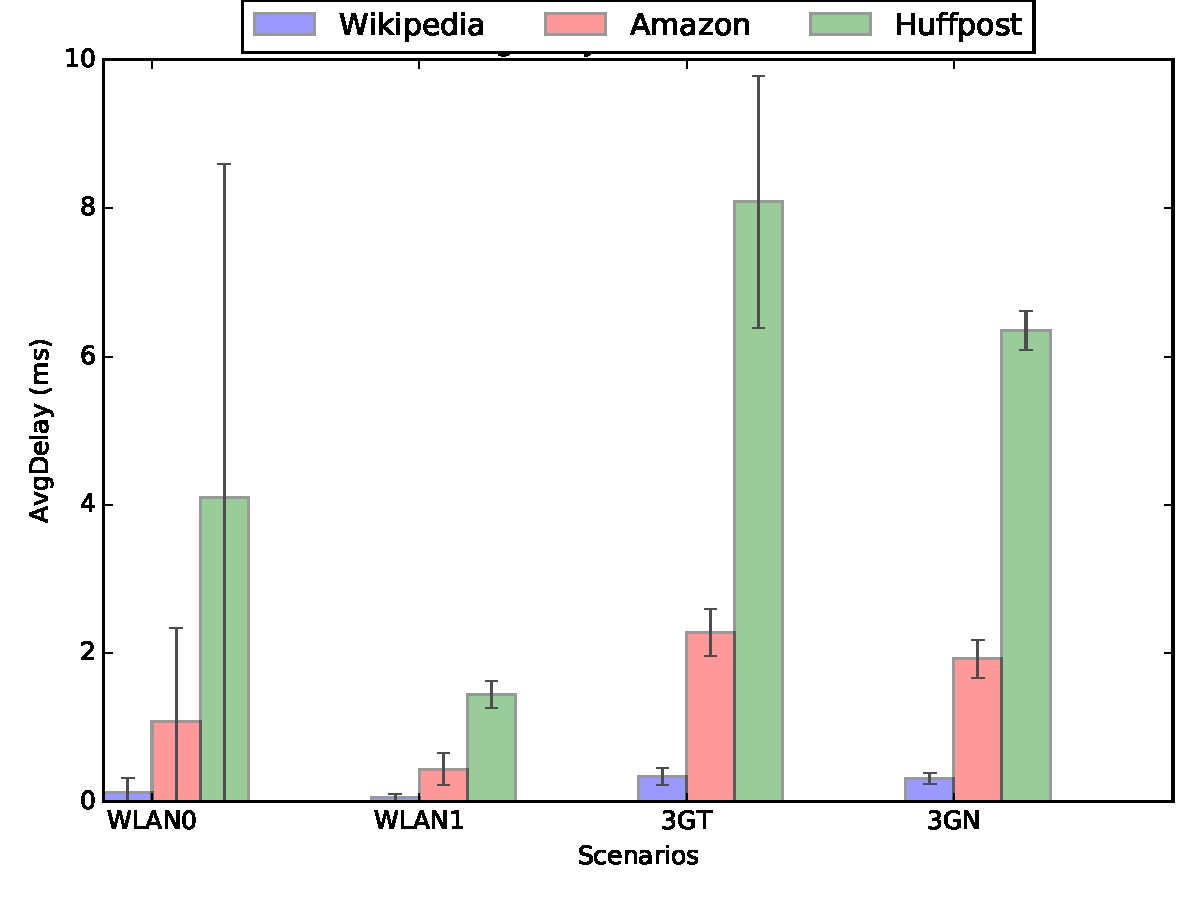
\includegraphics[width=.4\linewidth]{plots/NORNET-TCP-http.pdf}
  }
  \subfloat[Application Delay: MPTCP\label{fig:nornet_mptcp_http_appdelay}]
  {
    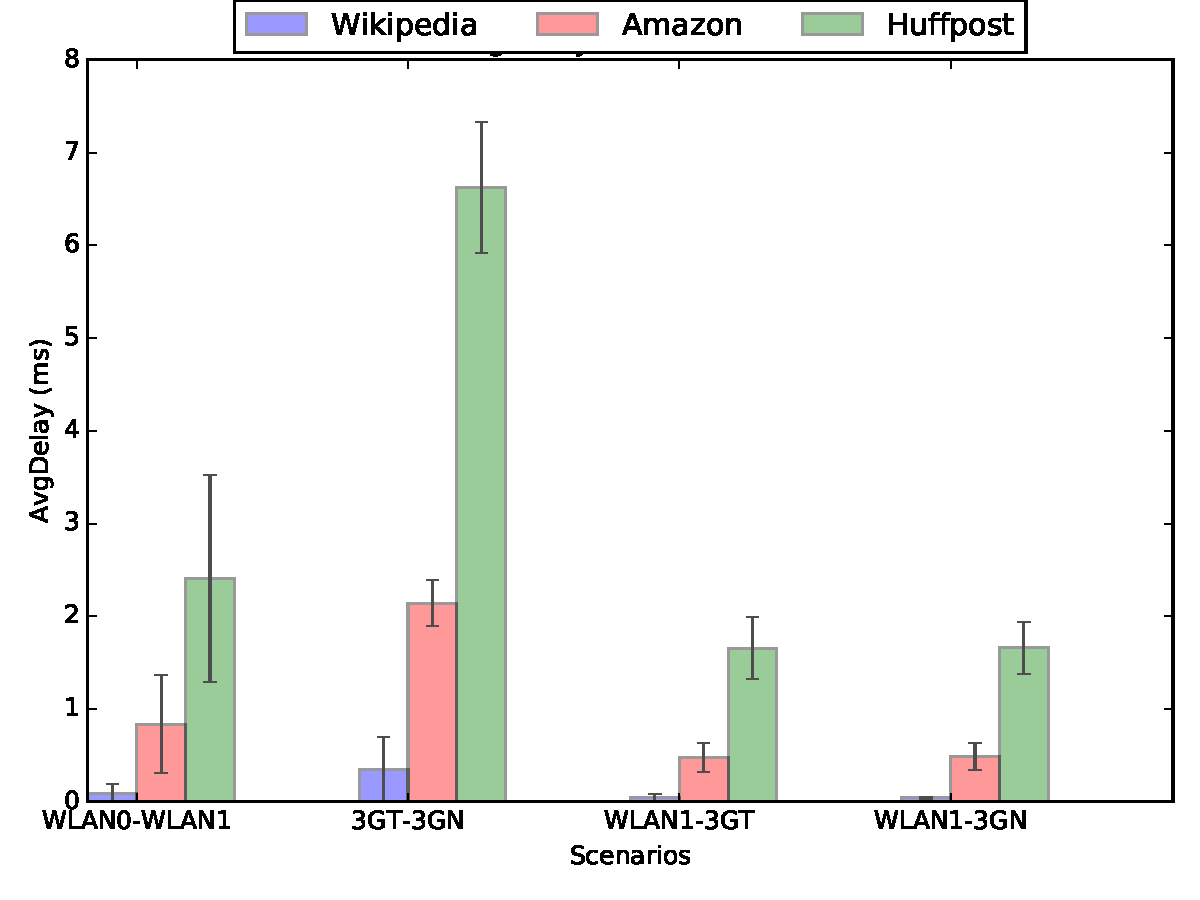
\includegraphics[width=.4\linewidth]{plots/NORNET-MPTCP-http.pdf}
  }
  \caption{Application delay with TCP and MPTCP and HTTP traffic: wikipedia, amazon and huffpost.}
  \label{fig:nornet_http_boxplot}
\end{figure*}

%Because we may drive
%biased conclusions if we evaluate the protocols in controlled environments only,
%we have also conducted experiments in a real life environment.

For the emulations, we use the Common Open
Research Emulator (CORE)~\cite{CORE}. The setup consists of two end-hosts, one acting as a mobile
device equipped with two interfaces and the other as a web server. To reach the
server, each interface of the mobile client is connected to an (emulated) access
network of its own. For the real-word experiments, we use the NorNet testbed~\cite{PAMS2013-NorNet} that consists of nodes that are simultaneously connected to multiple 3G operators in Norway as well as multiple public WLANs at Simula Research Laboratory. In our experiments, NorNet node act as the end-host and we use a web-server located in Oslo.

To evaluate the effect of having both homogeneous and heterogeneous network access we performed 3 sets of experiments where the interfaces used a combination of WLAN and 3G access (i.e., WLAN-WLAN, WLAN-3G, 3G-3G). For the emulations, the capacity of the WLAN was randomly chosen in the range 20-30Mbps, whereas for 3G we use values in the range 3-5Mbps. The propagation delays are choosen in the range of 20-25ms and 65-75ms for WLAN and 3G, respectively.

For each experiment, the server stores a small set of files from three different classes
of websites: Wikipedia, Amazon and Huffpost. Each website contains different number of objects of different sizes. Of the three, Wikipedia was the smallest ($15$ objects, $72$Kb total size) followed by Amazon ($54$ objects, $1$Mb total size) and then Huffpost ($138$ objects, $3.9$Mb total size). The sites were then requested and downloaded from the mobile client using six concurrent connections each using TCP or MPTCP, in respective
experiments.

We define the user experience of web browsing as the time needed to download a web page, hence, we measure the average flow completion time for each class of web page.

%There is a huge impact of the congestion level on the behavior of congestion
%control protocols~\cite{ha-background-traffic-comnet-2007}. We therefore conduct
%experiments both without and with background traffic.  The background traffic is
%a mix of TCP and UDP flows constituting one long TCP flow and 4 UDP flows. The
%aggregate usage of background flows maintained at 10\% of the bottleneck link
%capacity to be more realistic. The UDP flows carry data at 500kbps each in the
%WLAN-WLAN scenario and 100kbps each in the 3G-3G scenario.  In each run, the
%background flows start before the foreground experimental traffic and end after
%the experimental traffic.



%\per{change graph types to bar plots}
%
%\ozgu{need to make the figures similar in terms of format}

Figure~\ref{fig:web} shows the average transfer times for web traffic, with
standard variation over $30$ repetitions for each configuration without background traffic. Each figure depicts the average
transfer time when using MPTCP, TCP on one of the interfaces (TCP1, TCP2), or
TCP on the best available interface (MinTCP); the results are grouped according
to the emulated access networks used (WLAN-WLAN/3G-3G/WLAN-3G). We observe that MPTCP
cannot reduce transfer times for the Wikipedia site, but is able to do so for
both Amazon and Huffpost (especially in the 3G-3G scenarios). The reason for the
poor performance of retrieving the Wikipedia site is simply that
the amount of data is so small that it can be transmitted
within TCP's initial window (given the six concurrent connections used).
Employing more paths in such scenarios is not useful as long as the path itself
can sustain the traffic load. However, for the other sites the amount of data is
much larger and the transfer time can be reduced by MPTCP's implicit load-balancing
over its available subflows; the positive effects of this load-balancing peek
when the path characteristics of the subflows are homogeneous, as possible
head-of-line blocking effects are less prevalent.

%The top row
%contains results when no background traffic was present and the bottom row shows
%results with background traffic. 

%Eenabling background traffic
%(Figures~\ref{fig:web:wikipediawbg}-\ref{fig:web:huffpostwbg}) does not pose any
%major difference on the results, other than in absolute numbers.
%
%\per{something more about this :)}

%\per{maybe only mention the real experiments, and that they mostly confirm the
%emulated ones?}

% TODO: decide whether to include these graphs or just mention that they confirm
% the emulated (or vice versa but that's a counter intuitive approach)

Figure \ref{fig:nornet_http_boxplot} illustrates the average transfer times for web traffic for real-word experiments. For Wikipedia, consistent with the emulation results, we observe that MPTCP cannot reduce the latency. For Amazon, MPTCP performs very close to TCP while we observe lower download times for huffpost except for the (WLAN-WLAN) case.

%\srl{OA: Experiments are consistent with simulations except for the WLAN and WLAN case. It is probably due to our WLANs being very different.}

%\srl{OA: We should modify the figures to be similar to the emulation case, it is difficult to compare with the current figures.}

%We also illustrated the traffic distribution on different paths in Figure \ref{fig:nornet_http_barplot}. We observed that for heterogeneous cases, almost all traffic is carried over WLAN path whereas for the homogeneous cases,the distribution depends on the size of the website.
